\documentclass{standalone}
\usepackage{tikz}
\usepackage{amsmath}
\usepackage{fontspec}
\usetikzlibrary{snakes}

%: === TIPOGRAFÍA === (((
\setmainfont[
  BoldFont       = bodonibi,
	ItalicFont     = Century modern italic2.ttf,
	BoldItalicFont = bodonibi,
	SmallCapsFont  = lmromancaps10-regular.otf
]{Century_modern.ttf}
% )))

% === ENTRADA MATEMÁTICA === (((
\DeclareSymbolFont{italics}{\encodingdefault}{\rmdefault}{m}{it}
\DeclareSymbolFontAlphabet{\mathit}{italics}
\ExplSyntaxOn
\int_step_inline:nnnn { `A } { 1 } { `Z }
 {  \exp_args:Nf \DeclareMathSymbol{\char_generate:nn{#1}{11}}{\mathalpha}{italics}{#1} }
\int_step_inline:nnnn { `a } { 1 } { `z } {  \exp_args:Nf \DeclareMathSymbol{\char_generate:nn{#1}{11}}{\mathalpha}{italics}{#1}}
\ExplSyntaxOff
% )))

\begin{document}

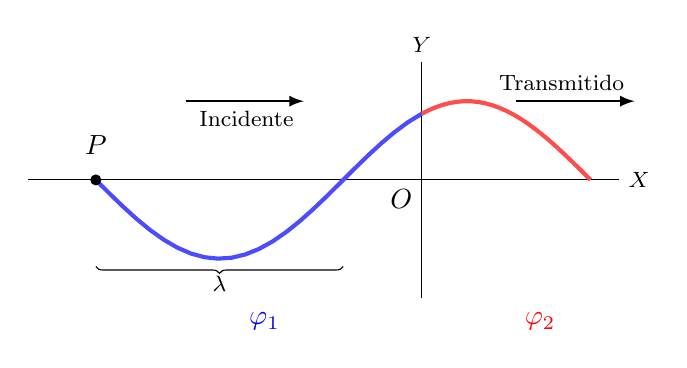
\begin{tikzpicture}[>=latex]
	\draw (-4,0) -- (3.5,0) node [right] {\footnotesize \(X\)};
	\begin{scope}[xshift=1cm]
		\draw (0,-1.5) -- (0,1.5) node [above] {\footnotesize \(Y\)};
		\node [below left] at (0,0) {\(O\)};
	\end{scope}
	\draw [line width = 1.5pt, blue!70, domain=-pi:1] plot(\x , {sin(\x r)});
	\draw [line width = 1.5pt, red!70, domain=1:pi] plot(\x , {sin(\x r)});
	\fill (-pi,0) circle (2pt) node [above=2mm] {\(P\)};
	\draw [thick,->] (-2,1) --++ (1.5,0) node [below left] {\footnotesize Incidente};
	\draw [thick,->] (2.2,1) --++ (1.5,0) node [above left] {\footnotesize Transmitido};
	\draw [snake = brace, mirror snake] (-pi,-1.1) to node[midway,below] {\footnotesize \(\lambda\)} (0,-1.1);
	\node [blue] at (-1,-1.8) {\(\varphi _1\)};
	\node [red] at (2.5,-1.8) {\(\varphi _2\)};
\end{tikzpicture}

\end{document}
